\chapter{Sequenzdiagramme}
Die folgenden Sequenzdiagramme sollen den Ablauf von einzelnen Anwendungsfällen im PaVoS-System illustrieren. Die Interaktionen der Klassen miteinander in verschiedenen Situationen wird somit verdeutlicht.

\section{Bridge}
In diesem Sequenzdiagramm wird der Ablauf der Bridge beschrieben, die MQTT-Nachrichten in Records umwandelt und diese an Kafka weiterleitet. Die Bridge läuft komplett unabhängig vom restlichen System.\\
Die Bridge kann sich in einer von drei Phasen befinden:
\begin{enumerate}
	\item \textbf{Aufbauphase:} Hier findet die Prüfung der Parameter und das Initialisieren der benötigten Klassen statt.
	\item \textbf{Bereitschaftsphase:} Hier ist die Bridge bereit, Nachrichten von MQTT anzunehmen, zu konvertieren und an Kafka weiter zu senden.
	\item \textbf{Abbauphase:} Hier werden die Verbindungen zu MQTT und Kafka getrennt, anschließend wird die Bridge beendet.
\end{enumerate}
In der Aufbauphase (in diesem Diagramm Operationen 1-5) wird zunächst ein \texttt{JmkbKafkaProducer} erstellt, der intern einen \texttt{KafkaProducer} mit bestimmten Einstellungen initialisiert und eine Verbindung zum Kafka Broker aufbaut. Danach wird ein \texttt{JmkbMqttConsumer} erstellt, der intern einen \texttt{MqttClient} mit bestimmten Einstellungen initialisiert, welcher eine Verbindung zum MQTT-Server aufbaut und die Topics abonniert, die vom FROST-Server angeboten werden.\\\\
Nun beginnt die Bereitschaftsphase. Sobald eine Nachricht beim MqttClient ankommt, wird die Methode \texttt{messageArrived} des \texttt{JmkbMqttConsumer}s aufgerufen. In dieser Methode wird aus der erhaltenen Nachricht die IOT-ID des Sensors gefiltert und die Nachricht wird in das Avro-Format konvertiert. Diese zwei Daten sind dann key und value für das Kafka \texttt{ProducerRecord} und werden über einen Aufruf der \texttt{send}-Methode des \texttt{JmkbKafkaProducer}s in ein solches Format gewandelt. Anschließend wird das Record durch den KafkaProducer an Kafka gesendet.\\\\
In der Abbauphase werden die \texttt{disconnect}-Methoden von \texttt{JmkbMqttConsumer} und \texttt{JmkbKafkaProducer} aufgerufen, die jeweils die Verbindungen zu MQTT und Kafka sauber trennen und die Clients schließen. Die Abbauphase beginnt nur dann, wenn der Nutzer des Programms es willkürlich schließt oder das System es beendet.
\begin{figure}[!hbp]
	\centering
	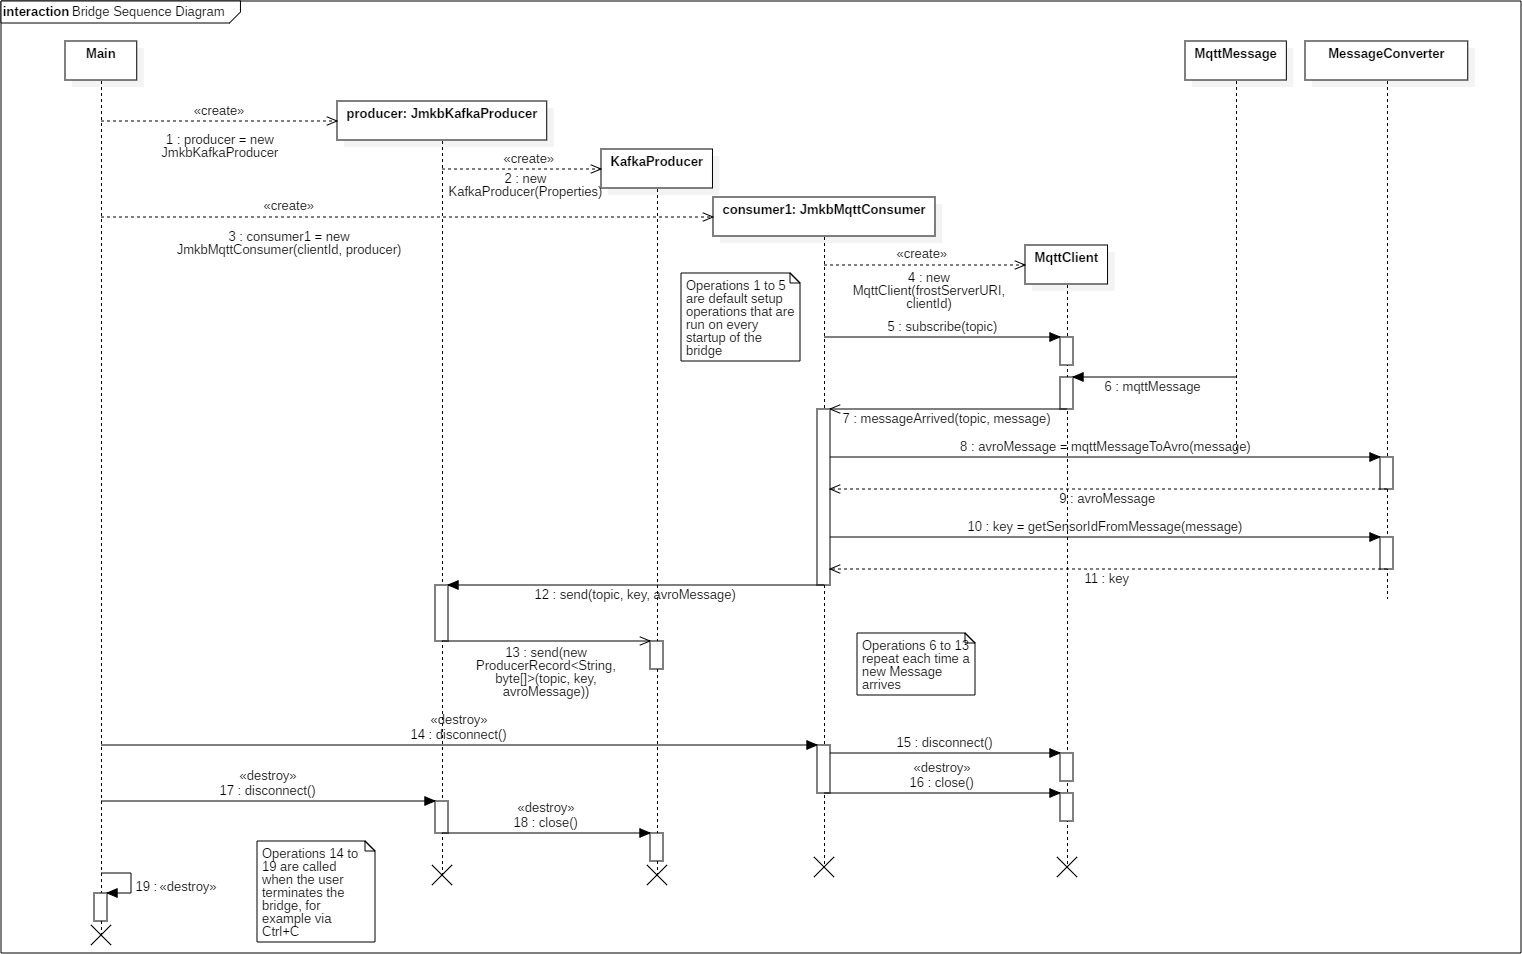
\includegraphics[width=\textheight,angle=90]{images/bridge/BridgeSequenceDiagram.png}
\end{figure}
\newpage

\section{Core}
Core
\begin{figure}[!hbp]
	\centering
	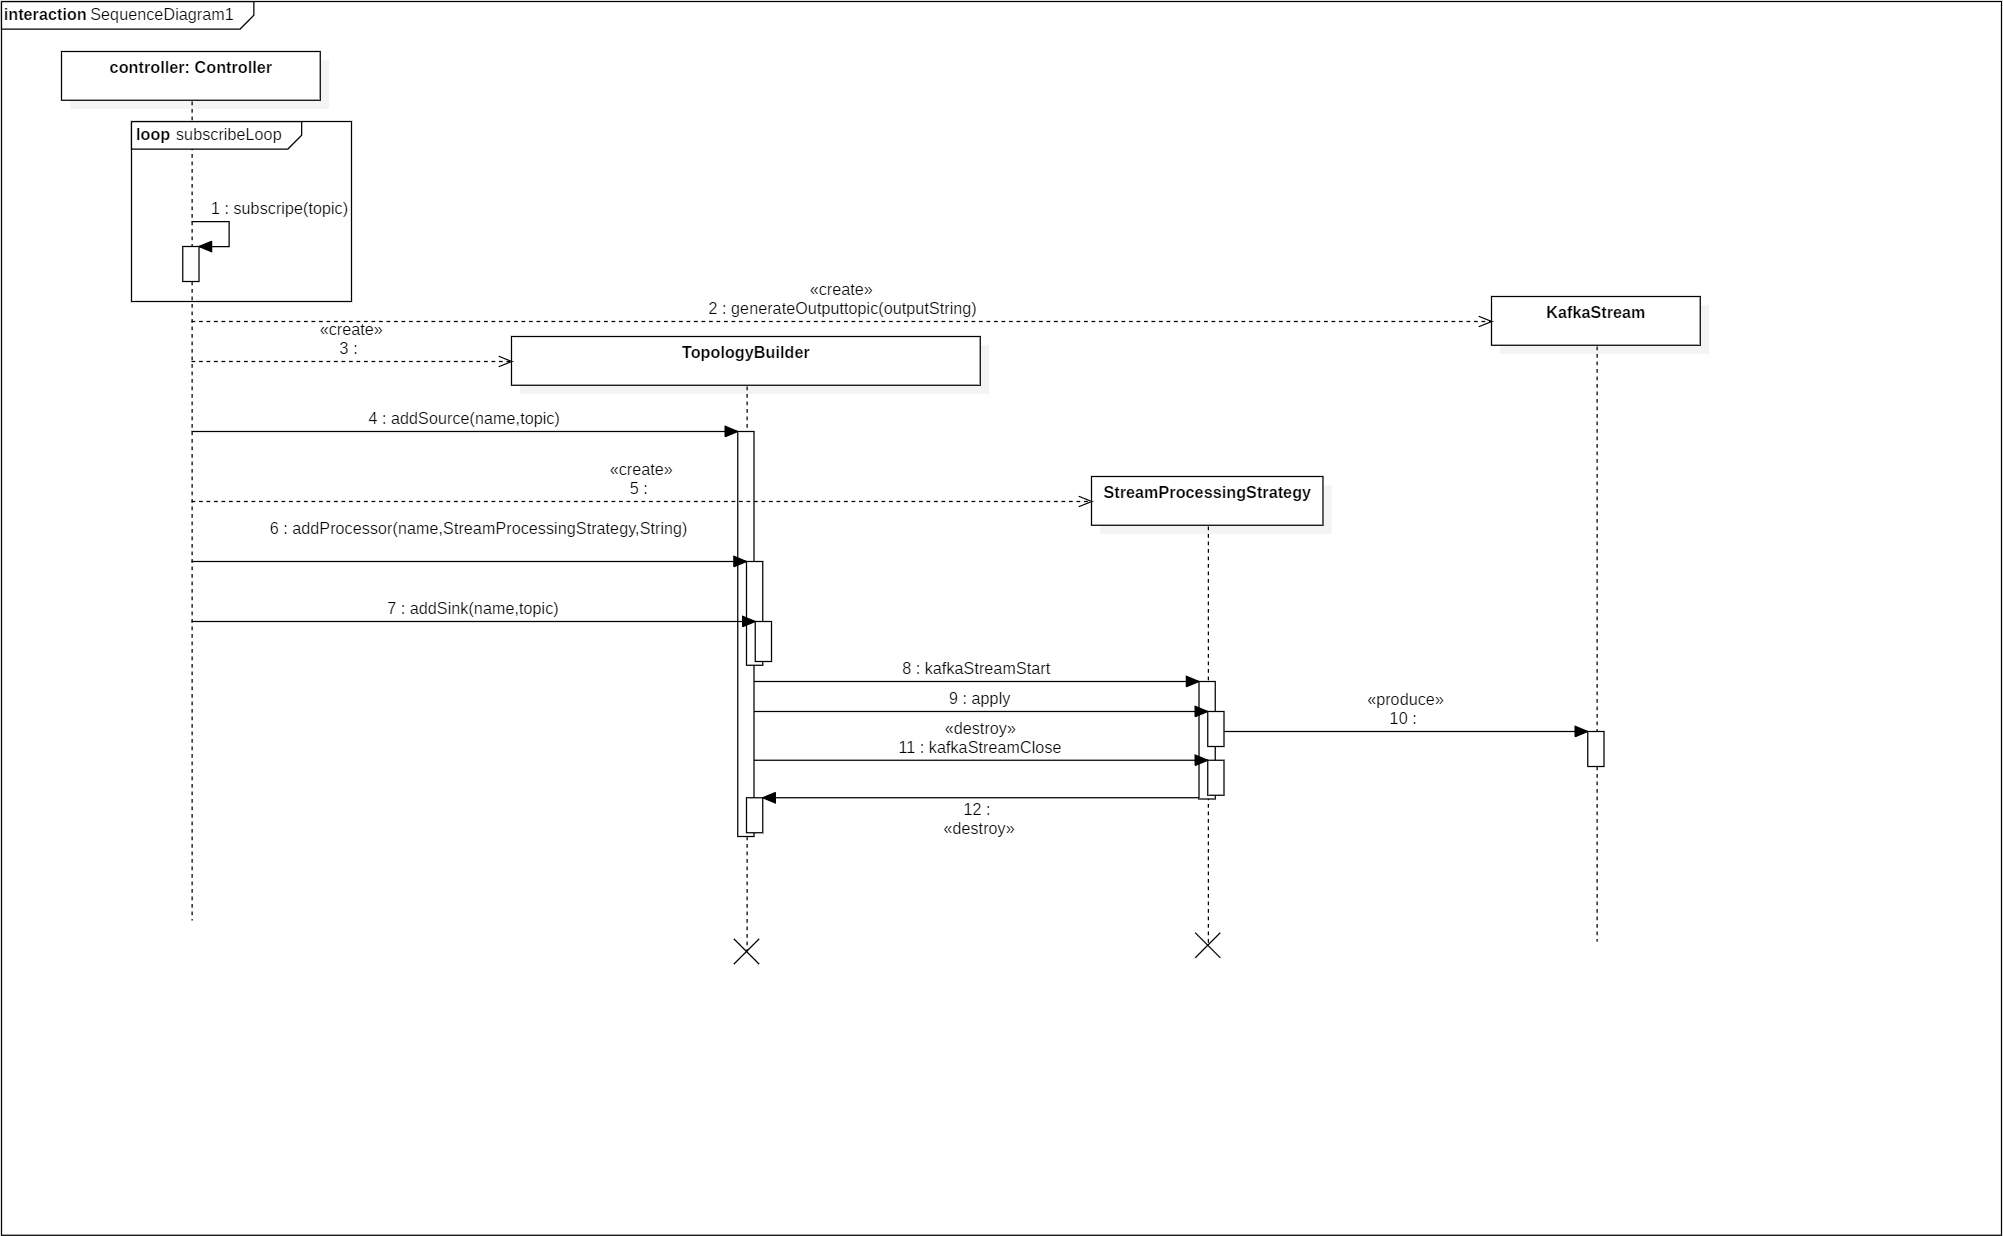
\includegraphics[width=\linewidth]{images/core/CoreSequenceDiagram.png}
\end{figure}
\newpage

\section{Import}
Import
\begin{figure}[!hbp]
	\centering
	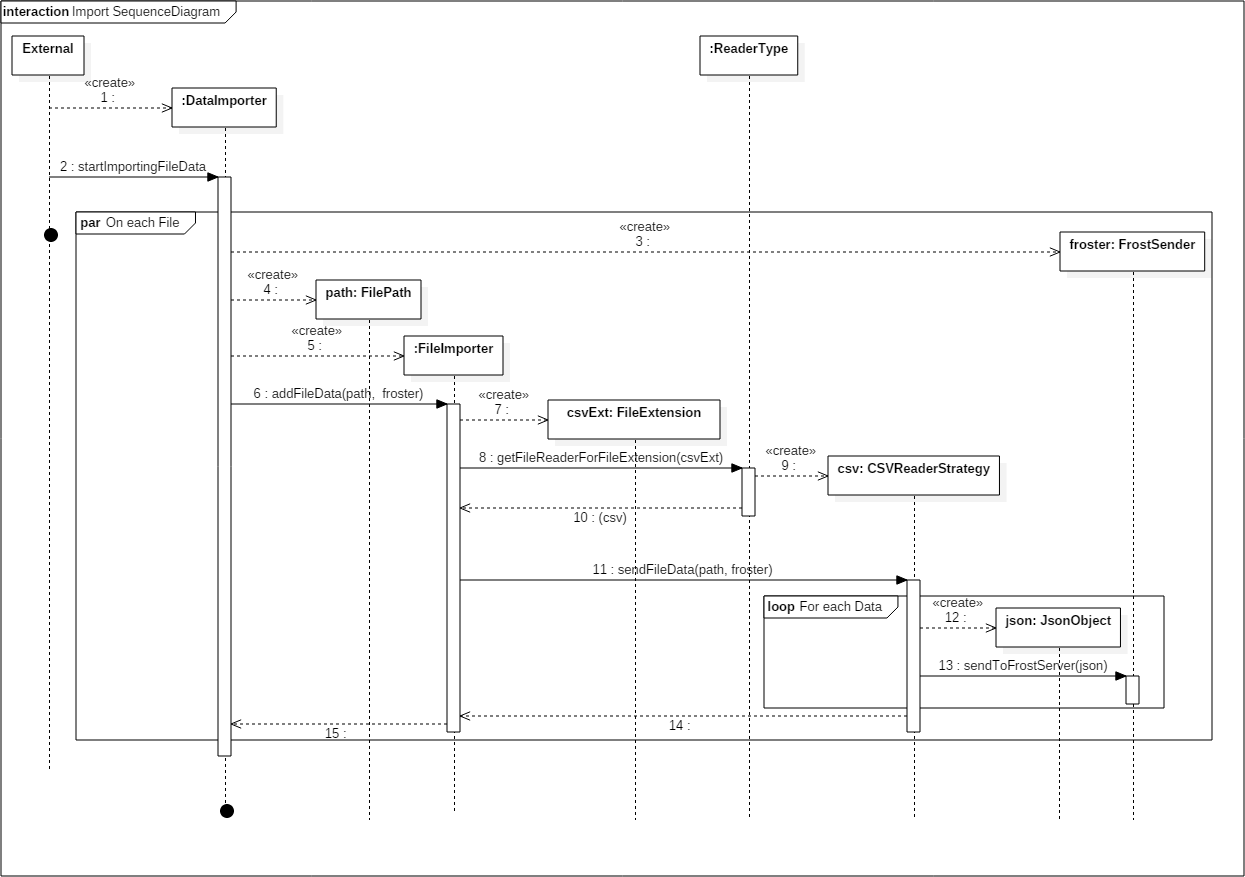
\includegraphics[width=\linewidth]{images/import/ImportSequenceDiagram.png}
\end{figure}
\newpage

\section{Graphite}
Graphite Main
\begin{figure}[!hbp]
	\centering
	\includegraphics[width=\linewidth]{images/graphite/GraphiteMainSequenceDiagram.png}
\end{figure}
\newpage
Graphite Sender
\begin{figure}[!hbp]
	\centering
	\includegraphics[width=\linewidth]{images/graphite/GraphiteSenderSequenceDiagram.png}
\end{figure}
\newpage

\section{Export}
Export
\begin{figure}[!hbp]
	\centering
	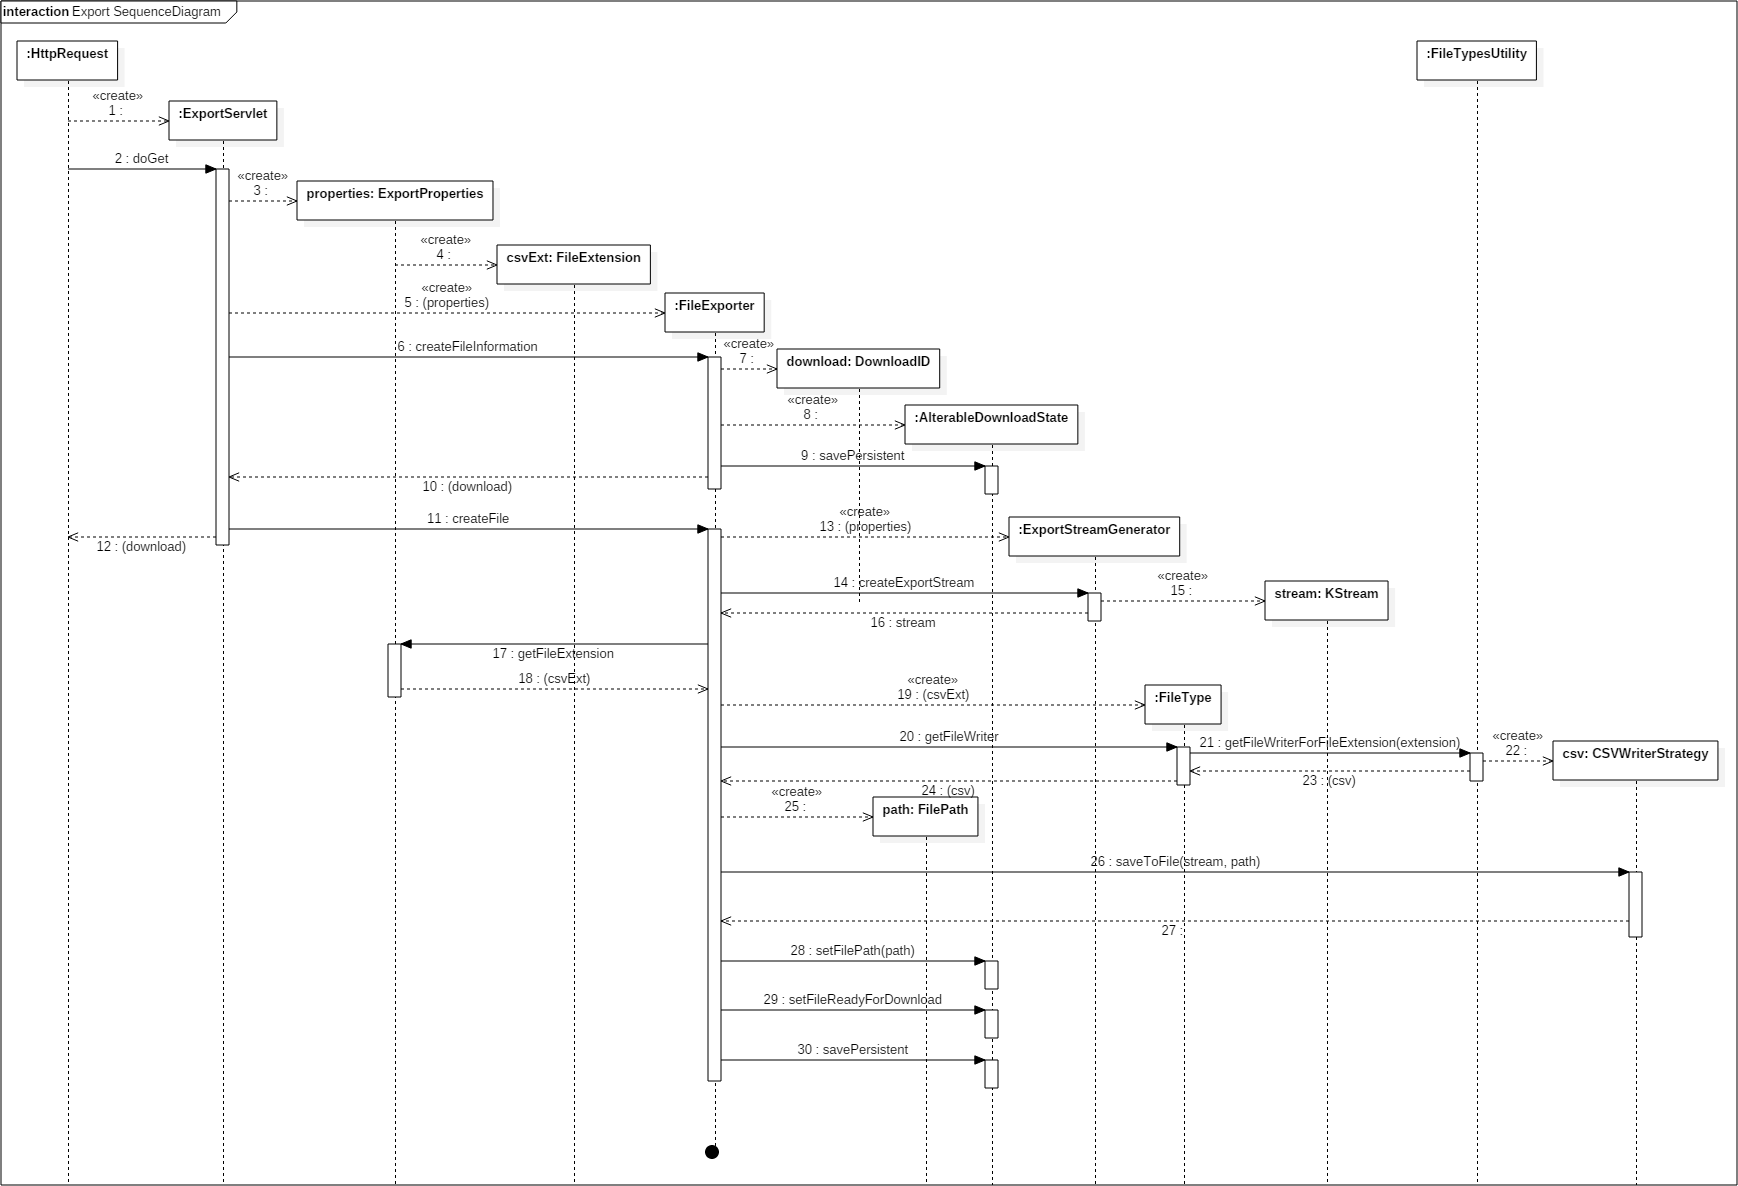
\includegraphics[width=\linewidth]{images/export/ExportSequenceDiagram.png}
\end{figure}
\newpage
Download
\begin{figure}[!hbp]
	\centering
	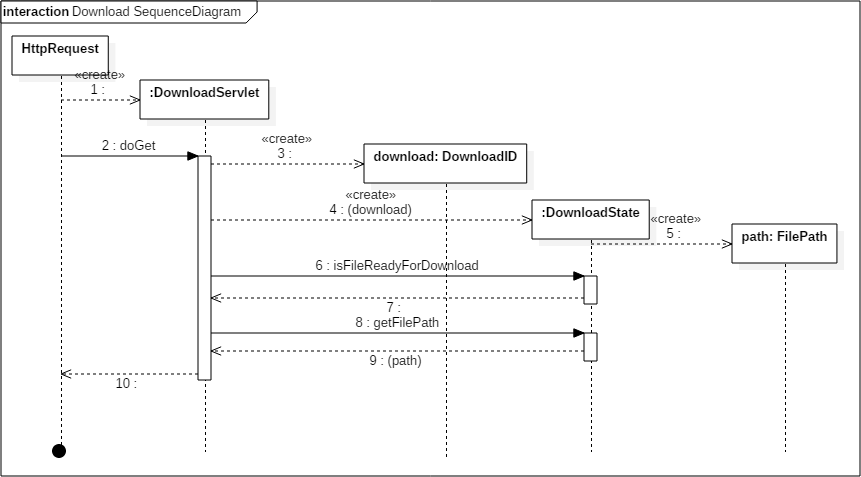
\includegraphics[width=\linewidth]{images/export/DownloadSequenceDiagram.png}
\end{figure}